\documentclass[12pt,letterpaper]{report}

\usepackage{amsfonts}
\usepackage{amssymb}
\usepackage{amsmath}
\usepackage{amsthm}
\usepackage{newlfont}
\usepackage[Glenn]{fncychap}
\usepackage{fancyhdr}
%\usepackage[ansinew]{inputenc}
\usepackage[utf8]{inputenc}
\usepackage{graphicx} % Para incluir imágenes
\usepackage{caption}  % Para manejar captions de manera personalizada

\captionsetup[figure]{
	justification=centering, % Alinea la descripción al lado izquierdo
	singlelinecheck=false,     % Evita centrar captions de una sola línea
	position=above,            % Coloca la descripción arriba
	labelfont={small,bf},
	labelsep=newline,
	textfont={small},
}
% Configuración específica para las notas
\DeclareCaptionLabelFormat{nolabel}{} % Define un formato sin etiqueta
\captionsetup*[figure]{
	textfont={Large}
}

\captionsetup[table]{
	justification=centering, % Alinea la descripción al lado izquierdo
	singlelinecheck=false,     % Evita centrar captions de una sola línea
	position=above,            % Coloca la descripción arriba
	labelfont={small,bf},
	labelsep=newline,
	textfont={small},
}
% Configuración específica para las notas
\DeclareCaptionLabelFormat{nolabel}{} % Define un formato sin etiqueta
\captionsetup*[table]{
	textfont={small}
}


\usepackage[spanish,mexico]{babel}
%% paquetes 
\usepackage{colortbl}
\usepackage{multicol}
\usepackage[colorlinks=true,linkcolor=black,urlcolor=black,citecolor=blue]{hyperref}
\usepackage[natbibapa]{apacite} % Paquete para citar en APA



\captionsetup[ruled]{width=0.5\textwidth,singlelinecheck=false,labelsep=newline,textfont={small}}

%--------------------%%Trazos y Logo de carátula

\usepackage{wallpaper}
\usepackage{pdflscape}
\usepackage[pages=some]{background}%all :para todas la páginas   some:Únicamente para algunas páginas
\backgroundsetup{
	scale=1,
	%color=black,
	opacity=1,
	angle=0,
	contents={
\includegraphics[width=\paperwidth,height=\paperheight]{Caratula4.pdf}}%
}
%--------------------



\textheight=9in %%Establece el largo del texto en cada página. El default es 19 cm.
\textwidth=6.5in %%Establece el ancho del texto en cada página . El default es 14 cm.
\topmargin=-1.2cm %%%Establece el margen superior.  A margin width of 0cm gives you a margin 4cm wide
\oddsidemargin=-.5cm %%Establece el margen izquierdo de la hoja. El default es de 4.5 cm; sin embargo, con sólo poner esta instrucción el margen queda en 2.5 cm. Si el parámetro es positivo se aumenta este margen y si es negativo disminuye.
\setlength{\topskip}{0.3in}    % between header and text

\oddsidemargin=0cm %margen para páginas impares se necesita twoside en \documentclass de otro modo es irrelevante el comando
\evensidemargin=0cm %margen para páginas pares se necesita twoside en \documentclass de otro modo es irrelevante el comando



\renewcommand{\baselinestretch}{1.1}

\usepackage{setspace}
\setlength{\parindent}{24pt}
\setlength{\parskip}{14pt plus3pt minus4pt}



\parindent=0mm %%Elimina Sangria

\newcommand{\R}{\mathbb R}
\newcommand{\N}{\mathbb N}
\newcommand{\C}{\mathbb C}

% THEOREMS ---------------------------------------------------------------
\theoremstyle{plain}
\newtheorem{thm}{Teorema}[section]
\newtheorem{cor}[thm]{Corolario}
\newtheorem{lem}[thm]{Lema}
\newtheorem{obs}{Observación}[section]



\makeatletter
\renewcommand*{\cleardoublepage}{\clearpage\if@twoside
\ifodd\c@page\else
\hbox{}\thispagestyle{empty}\newpage
\if@twocolumn\hbox{}\newpage\fi\fi\fi}
\makeatother


%\setlength{\parskip}{8mm}%Espacio entre párrafos. Por defecto \parskip tiene asignado 0 que es un espacio igual al de el espacio entre líneas.

\usepackage{enumitem}
\usepackage[utf8]{inputenc}
\usepackage[T1]{fontenc}
\usepackage[spanish]{babel}
\usepackage{xcolor}
\usepackage{graphicx}
\usepackage{multirow}
\usepackage{booktabs}
\usepackage{amsmath}
\usepackage{booktabs}
\usepackage{longtable}
\usepackage{array}

\newcommand{\corregido}[1]{\textcolor{blue}{#1}} % Comando para resaltar correcciones

\begin{document}

% ------------------------------------------------------------------------
 \pagestyle{empty}
 \BgThispage%%%para colocar el fondo de la carátula
 \LARGE

 \hspace{2.8cm}
\begin{minipage}[l]{15cm}
\begin{center}
\textbf{\textit{\textcolor[rgb]{0.30,0.04,0.04}{Universidad Autónoma de Tlaxcala}}}
\end{center}

%\vspace{1cm}
 \Large
\begin{center}
\emph{\textcolor[rgb]{0.43,0.00,0.00}{Facultad de Ciencias  Básicas, Ingeniería y Tecnología}}
\end{center}
\vspace{2cm}
\begin{center}
\textbf{ ``Análisis de datos de bioseñales con el lenguaje de programación Python'' }
\end{center}
\vspace{1.2cm}

\begin{center}
\textbf{TESIS}

 \vspace{1.2cm}

Que para obtener el grado de:

 \textbf{Licenciado en Matemáticas Aplicadas}

\vspace{1.2cm}

 Presenta:

Said Tecpa Juárez
\end{center}
\vspace{.5cm}

\begin{center}
Director de Tesis:

M. en C. Roberto Rosales Flores
\end{center}


\begin{center}
Asesora de Tesis:

Dra. Dora Luz Corona Quintanilla
\end{center}

\end{minipage}

\vfill{
\begin{flushright}
\normalsize
Apizaco, Tlaxcala,   20\_\_.
\end{flushright}
}


%% -----------------------------------------------------------
\normalsize
%
%
\pagestyle{empty}

Hoja de liberaci\'on 
%
\thispagestyle{empty}
\setcounter{page}{0}

\hfill\emph{Dedicatoria (opcional)}

\noindent \textcolor[rgb]{0,0,1}{En esta sección tienes la libertad de nombrar a las personas a las que les ofrecerás como tributo tu esfuerzo, pero sé mesurado en los elogios. No te excedas de una página.  Sé creativo y sincero.}

\noindent \textcolor[rgb]{0,0,1}{Ejemplo:\newline
	A mi esposa y a mis hijos, por su paciencia y amor.\newline
	A todos mis hermanos, extraordinarios maestros y compañeros de vida.\newline
	A mis compañeros de licenciatura. Siempre los recordaré con alegría.}

%\chapter*{Agradecimientos}
\thispagestyle{empty}
\setcounter{page}{0}

\noindent \textcolor[rgb]{0,0,1}{Mientras que las dedicatorias se destinan a familiares y amigos, este apartado se reserva para mostrar tu gratitud, ya sea a tu centro de trabajo por las facilidades brindadas para la terminación de tus estudios, o a la institución educativa que te otorgará el título. Puedes referirte a una persona en particular y explicar de manera sintética los motivos. Sé mesurado. No entrecomilles ninguna parte para evitar que tu comentario se entienda como una ironía.}

\noindent \textcolor[rgb]{0,0,1}{Ejemplo:\newline
	A lo largo de un trabajo de amplia duración, ...\newline
	A todos ellos quiero mostrarles mi más sincero agradecimiento.}

\pagestyle{plain}
\pagenumbering{roman}
%\chapter*{Resumen}
\markboth{RESUMEN}{\small RESUMEN}
\addcontentsline{toc}{chapter}{Resumen}

\setcounter{page}{1}
\noindent El presente trabajo muestra una metodología para preparar a los alumnos en la aplicación de pruebas estandarizadas, \corregido{en particular para mejorar} los resultados de la prueba PLANEA. \corregido{Se incluye} información teórico-conceptual sobre evaluación y su importancia para medir el desempeño académico \corregido{de los sistemas educativos} en diferentes países, en particular en México, a través de la prueba PLANEA.

\noindent Se plantea \corregido{un método} de mejora de los resultados mediante la implementación de \corregido{un banco de ejercicios} donde el alumno encuentre \corregido{un recurso} de trabajo para prepararse \corregido{previamente} antes de ser aplicada la prueba. \corregido{Se empleó} la metodología ADDIE, \corregido{mediante} procesos que incluyen \corregido{las fases de} análisis, diseño, desarrollo, implementación y evaluación.

\noindent Se recabó información de las pruebas PLANEA 2016 y 2017 para \corregido{organizar} los reactivos y \corregido{clasificarlos} en ejes, niveles y asignaturas \corregido{según los estándares de} PLANEA MS. Con esta información se construyó \corregido{un banco} de ejercicios tipo PLANEA y se propuso \corregido{un protocolo} de aplicación.

\noindent Para verificar \corregido{la efectividad} del \corregido{banco de ejercicios}, se llevó a cabo \corregido{una evaluación comparativa} diagnóstica y final. Los resultados se interpretaron a través de tablas y gráficas elaboradas por niveles de desempeño, \corregido{y se aplicó} la prueba de hipótesis $t$ de Student para \corregido{comparar las medias por niveles y determinar} si hubo una mejora \corregido{significativa} en los resultados.
\tableofcontents
\listoffigures
\listoftables

\pagestyle{fancy}
\fancyhead[RE]{ }% deja vacío el encabezado derecho de páginas pares.
\fancyhead[LO]{ }% deja vacío el encabezado izquierdo de páginas impares.
\pagenumbering{arabic}
% ------------------------------------------------------------------------
\chapter*{Introducción}
\markboth{INTRODUCCIÓN}{\small INTRODUCCIÓN}
\addcontentsline{toc}{chapter}{Introducción}
\setcounter{page}{1}


\noindent La evaluación educativa es un tema importante a nivel mundial. Los gobiernos \corregido{de distintos países,} preocupados por este tema, recurren a diversos organismos nacionales e internacionales como la Asociación Internacional para la Evaluación del Rendimiento Educativo (IEA), la Organización para la Cooperación y el Desarrollo Económico (OCDE) o la Comisión Nacional para la Mejora Continua de la Educación (MEJOREDU), \corregido{los cuales aplican} pruebas como TIMSS, PISA o PLANEA, \corregido{que} tienen como objetivo conocer el estado \corregido{actual de} la educación en cada país.

\noindent En México, desde 2006 \corregido{con} la prueba ENLACE, \corregido{existía} un mecanismo que permitía conocer información diagnóstica del nivel de logro académico \corregido{en} las asignaturas de español y matemáticas, \corregido{que fue sustituida} por PLANEA en 2015.

\noindent Los resultados en México \corregido{en estas pruebas} han sido bajos, \corregido{con la mayoría ubicados} en el nivel I. Esto representa una preocupación para las instituciones educativas, \corregido{que} consideran \corregido{estos resultados como} un reto \corregido{y un} desafío para la educación media superior. A pesar de la importancia de estas evaluaciones, desde 2022 \corregido{no se han aplicado} pruebas estandarizadas como PLANEA o PISA; \corregido{sin embargo, este es un tema que no debe perderse de vista.}

\noindent En el presente trabajo de tesis, se aborda esta problemática \corregido{buscando} una estrategia para mejorar el desempeño de los estudiantes, mediante el diseño e implementación de una propuesta didáctica \corregido{que mejore su desempeño} en la resolución de reactivos tipo PLANEA en Educación Media Superior. En particular, se trabajó con estudiantes del plantel 06 de Contla, en el campo disciplinar de cálculo integral \corregido{de} sexto semestre.

\noindent \corregido{A modo de guía, a continuación se describe la estructura del trabajo de tesis:}

\noindent En el \textbf{Capítulo 1} se presenta el planteamiento del problema, las preguntas de investigación, los objetivos, la hipótesis y la justificación.

\noindent El \textbf{Capítulo 2} expone la parte metodológica, \corregido{incluyendo} conceptos como: evaluación, tipos de evaluación, examen, prueba, tipos de reactivos, aprendizaje esperado, \corregido{además de} información relevante sobre la prueba PLANEA, sus propósitos, consideraciones metodológicas, niveles de logro, \corregido{su} relación con el marco curricular común \corregido{y aspectos de} diseño instruccional.

\noindent El \textbf{Capítulo 3} describe la aplicación del método ADDIE (Análisis, Diseño, Desarrollo, Implementación y Evaluación) \corregido{detallando} cada fase. \corregido{Se analizan} las pruebas PLANEA 2016, 2017 y 2020, \corregido{construyéndose} tablas que clasifican los reactivos según su eje temático, el tema correspondiente en el programa de estudios del campo disciplinar de matemáticas de la Dirección General de Bachillerato (DGB) y el número de reactivos por tema. \corregido{La última sección especifica el} lugar donde se realizó la investigación.

\noindent El \textbf{Capítulo 4} presenta los resultados de la implementación \corregido{del material}, \corregido{los resultados} de la evaluación aplicada a los alumnos \corregido{y su} análisis para determinar el nivel de logro.

\noindent Finalmente, el \textbf{Capítulo 5} establece la validación de la hipótesis, las conclusiones, hallazgos \corregido{y} recomendaciones.
\chapter{Objeto de la investigación}
\markboth{CAPÍTULO 1. OBJETO DE LA INVESTIGACIÓN}{\small CAPÍTULO 1. OBJETO DE LA INVESTIGACIÓN}
\label{ObjetoInv}
 
\parskip=12pt
\section{Planteamiento del problema}\label{Seccion11}
\noindent La resolución de sistemas de ecuaciones lineales constituye un componente fundamental en el estudio del álgebra lineal, con aplicaciones esenciales en campos como la ingeniería, la física, la estadística y las ciencias computacionales. Entre los métodos más eficientes y ampliamente utilizados para resolver estos sistemas destacan las técnicas de factorización matricial, específicamente $\mathrm{LU}$, $\mathrm{LL^T}$ (Cholesky) y $\mathrm{LDL^T}$. Estas técnicas permiten descomponer matrices complejas en productos matriciales más simples, lo que facilita el cálculo, la manipulación algebraica y la interpretación de los sistemas.

\noindent No obstante, la enseñanza y el aprendizaje de estos métodos presentan desafíos significativos en los niveles medio superior y superior. Los estudiantes no solo deben internalizar algoritmos complejos, sino también comprender la abstracción que implica la notación matricial y la lógica algebraica subyacente a cada procedimiento. En muchos contextos académicos, la instrucción se limita a exposiciones teóricas acompañadas de ejercicios manuales, predominando un enfoque estático y poco interactivo que dificulta la conexión entre teoría y práctica.

Pese al creciente uso de tecnologías educativas en diversas áreas, se observa una notable carencia de herramientas digitales especializadas en la enseñanza interactiva de la factorización matricial. La mayoría de los recursos disponibles se centran en resolver sistemas lineales de manera automática o en aspectos algebraicos más generales, sin ofrecer una experiencia que permita visualizar detalladamente las matrices $\mathrm{L}$, $\mathrm{U}$ y $\mathrm{D}$, ni la posibilidad de manipular libremente los datos o validar paso a paso los resultados intermedios, aspectos fundamentales para consolidar el aprendizaje.

\parskip=15pt
\noindent Esta deficiencia afecta la comprensión conceptual de los estudiantes, quienes frecuentemente desconocen cómo se construyen las matrices de descomposición, cómo validar la factorización y cómo aplicar estos procesos para resolver eficazmente el sistema original. Por ello, resulta imperativo desarrollar un recurso digital que permita la interacción activa con los procedimientos, la exploración guiada y la retroalimentación inmediata, elementos que favorecen la motivación, el razonamiento crítico y la adquisición de un conocimiento profundo y duradero.

\noindent En consecuencia, el diseño de un programa con una interfaz clara, amigable e intuitiva que guíe al estudiante durante todas las etapas de la factorización matricial se perfila como una solución educativa viable. Esta herramienta deberá incluir funcionalidades para la validación manual de resultados intermedios, la representación explícita de las transformaciones matriciales y la experimentación con distintos conjuntos de datos, fomentando así un aprendizaje constructivo, significativo y adaptado a las necesidades y ritmos individuales.

\section{Justificación}

\noindent En el contexto actual de la educación matemática, se reconoce el papel fundamental que desempeñan los recursos digitales interactivos para facilitar la enseñanza y el aprendizaje de conceptos complejos y abstractos. El álgebra lineal, por su naturaleza, puede beneficiarse significativamente de software educativo que combine elementos visuales, interactividad y retroalimentación inmediata, características que fomentan un aprendizaje activo, la autonomía del estudiante y el desarrollo de habilidades analíticas y metacognitivas.

El presente proyecto propone el desarrollo de un programa interactivo, implementado en Python con bibliotecas gráficas como Tkinter o PyQt, que facilite el aprendizaje de los métodos de factorización $\mathrm{LU}$, $\mathrm{LL^T}$ y $\mathrm{LDL^T}$. Esta aplicación permitirá a los usuarios introducir sistemas personalizados, seguir detalladamente cada etapa de la factorización, visualizar las matrices generadas y validar manualmente los resultados, recibiendo retroalimentación automática y didáctica que corrija errores y refuerce conceptos clave.

\noindent Con esta propuesta se pretende abordar una necesidad educativa específica: superar la memorización mecánica de algoritmos para alcanzar una comprensión profunda y lógica de los procesos matriciales. Un entorno interactivo que fomente la experimentación y la autoverificación contribuye al desarrollo de competencias críticas, como la interpretación precisa de resultados, la toma de decisiones fundamentadas y el pensamiento estructurado.

\noindent Además, el diseño flexible y accesible del programa lo hace adecuado tanto para entornos presenciales como virtuales, pudiendo utilizarse como apoyo didáctico en clases o como herramienta para el autoaprendizaje. La elección de un lenguaje de programación abierto garantiza que el recurso sea gratuito, modificable y adaptable, lo que favorece la democratización del acceso a materiales educativos especializados y la mejora continua basada en la retroalimentación de estudiantes y docentes.

\noindent En síntesis, este proyecto constituye una contribución relevante a la innovación pedagógica en la enseñanza del álgebra lineal, integrando tecnología, interactividad y fundamentos didácticos. Se espera que esta iniciativa fortalezca la comprensión conceptual, incremente la motivación y mejore el rendimiento académico en un área fundamental del currículo matemático.

\section{Objetivos}

\subsection{Objetivo general}

\noindent Desarrollar un programa con interfaz interactiva que facilite de manera integral la enseñanza y el aprendizaje de la resolución de sistemas de ecuaciones lineales mediante métodos de factorización matricial $\mathrm{LU}$, $\mathrm{LL^T}$ (Cholesky) y $\mathrm{LDL^T}$. Este programa ofrecerá una guía estructurada, clara y paso a paso para el estudiante, incorporando validaciones automatizadas y retroalimentación continua que fortalezcan la comprensión tanto conceptual como práctica de los métodos. De esta forma, se fomentará un aprendizaje activo, significativo y autónomo, que desarrolle la capacidad de razonamiento matemático.

\subsection{Objetivos específicos}

\begin{itemize}
	\item Diseñar una interfaz gráfica intuitiva y accesible que permita a los usuarios ingresar matrices y vectores de manera sencilla, flexible y segura, facilitando la exploración, manipulación y experimentación con diferentes conjuntos de datos. La interfaz deberá incluir visualizaciones dinámicas y didácticas de las matrices resultantes $\mathrm{L}$, $\mathrm{U}$ y $\mathrm{D}$, así como de las etapas intermedias del proceso, con el fin de promover una comprensión profunda y visual del algoritmo.
	
	\item Implementar eficientemente los algoritmos de factorización $\mathrm{LU}$, Cholesky ($\mathrm{LL^T}$) y $\mathrm{LDL^T}$, asegurando el manejo correcto de matrices compatibles en dimensiones y propiedades algebraicas (como simetría, definida positiva y no singularidad). El programa incorporará validaciones internas rigurosas para prevenir errores numéricos comunes, garantizar estabilidad computacional y manejar adecuadamente casos especiales.
	
	\item Incorporar un sistema integral de retroalimentación automatizada y validación manual que permita al estudiante verificar sus cálculos en cada fase del proceso, detectar posibles errores o inconsistencias, y recibir sugerencias didácticas personalizadas que faciliten la corrección, la reflexión y el reforzamiento del aprendizaje autónomo y metacognitivo.
	
	\item Evaluar el impacto educativo del software mediante pruebas piloto con estudiantes de nivel superior, empleando instrumentos cuantitativos (pruebas de comprensión, evaluaciones de desempeño) y cualitativos (encuestas de opinión, entrevistas) para medir mejoras en la comprensión conceptual, retención de conocimientos, actitud hacia el aprendizaje y usabilidad del programa. Los resultados permitirán ajustar y optimizar la herramienta según las necesidades reales de los usuarios finales.
	
	\item Elaborar un manual que incluya guías detalladas de uso, ejemplos prácticos contextualizados para facilitar la integración efectiva del programa en los planes de estudio. Este material apoyará tanto a docentes que deseen incorporar la herramienta en su práctica educativa, como a estudiantes que utilicen el software de forma autónoma o en modalidades de autoaprendizaje.
\end{itemize}

\section{Hipótesis y preguntas de investigación}

\subsection{Hipótesis}

\noindent La implementación y uso de un programa interactivo diseñado para guiar la resolución de sistemas de ecuaciones lineales mediante factorización matricial ($\mathrm{LU}$, $\mathrm{LL^T}$, $\mathrm{LDL^T}$) mejora significativamente la comprensión conceptual, el aprendizaje activo y la retención a largo plazo de los conceptos matemáticos involucrados. Esta mejora se refleja en un mejor desempeño académico y una mayor motivación hacia el estudio del álgebra lineal, en comparación con metodologías tradicionales basadas exclusivamente en exposiciones teóricas y resolución de ejercicios estáticos sin apoyo tecnológico.

\subsection{Preguntas de investigación}

\begin{enumerate}
	\item ¿Qué características de la interfaz gráfica contribuyen de manera más efectiva a facilitar el aprendizaje y la comprensión de los métodos de factorización matricial?
	
	Esta pregunta busca identificar qué elementos visuales (por ejemplo: colores, diagramas), funcionalidades interactivas (validación inmediata, manipulación directa de matrices) y niveles de complejidad favorecen la experiencia educativa y la apropiación del conocimiento por parte de los estudiantes.
	
	\item ¿Cómo influye la retroalimentación automatizada y la validación manual en el proceso de aprendizaje de los estudiantes?
	
	Se pretende analizar si el feedback inmediato sobre errores o aciertos estimula la reflexión crítica, la autoevaluación, la motivación para corregir errores y la profundización en los conceptos, favoreciendo un aprendizaje autónomo, significativo y perdurable.
	
	\item ¿Cuál es el impacto real del uso del software en los niveles de comprensión y desempeño académico de los estudiantes en álgebra lineal?
	
	Esta interrogante está orientada a medir, mediante evaluaciones diagnósticas y sumativas, así como encuestas y entrevistas, la efectividad del programa como recurso educativo en comparación con métodos tradicionales de enseñanza.
	
	\item ¿En qué contextos educativos (presencial, semipresencial, a distancia) resulta más efectiva la integración del programa para el aprendizaje de la factorización matricial?
	
	Se busca determinar las condiciones y modalidades de enseñanza en las que la herramienta tecnológica aporta mayores beneficios pedagógicos, identificando limitaciones y potencialidades según el entorno educativo, la infraestructura tecnológica disponible y el perfil de los estudiantes.
\end{enumerate}

\goodbreak


 \chapter{Marco Teórico: Álgebra lineal y métodos de factorización matricial}
 \markboth{CAPÍTULO 2. Marco Teórico: Álgebra Lineal y Métodos de Factorización Matricial}{\small CAPÍTULO 2. Marco Teórico: Álgebra Lineal y Métodos de Factorización Matricial}
 \label{MarcoTeorico}

\section{Álgebra lineal}

\noindent El \textbf{álgebra lineal} constituye una rama fundamental de las matemáticas que estudia estructuras como vectores, espacios vectoriales, matrices y transformaciones lineales. Su relevancia trasciende el ámbito teórico, extendiéndose a numerosas aplicaciones en ciencia, tecnología e ingeniería. Representa la base de múltiples técnicas computacionales modernas, desde el análisis numérico hasta el aprendizaje automático, incluyendo el modelado de sistemas físicos, financieros y estadísticos.

Desde una perspectiva educativa, el álgebra lineal frecuentemente representa el primer contacto de los estudiantes con las matemáticas abstractas. La transición desde el álgebra elemental --centrada en ecuaciones y manipulaciones simbólicas-- hacia un pensamiento más estructurado requiere un cambio cognitivo significativo. La abstracción inherente a las matrices, los vectores en espacios de dimensión arbitraria y la interpretación de operaciones como transformaciones lineales puede dificultar el aprendizaje si no se complementa con estrategias pedagógicas adecuadas.

Diversos autores (Dorier, Robert, Robinet \& Rogalski, 2000; Harel \& Kaput, 1991) han señalado que los enfoques tradicionales de enseñanza del álgebra lineal suelen enfatizar excesivamente los procedimientos algebraicos, sin establecer conexiones suficientes con la visualización geométrica, la interpretación conceptual o las aplicaciones prácticas. Como respuesta a esta problemática, se ha impulsado el desarrollo de estrategias didácticas basadas en la interacción, la visualización y la experimentación guiada mediante recursos digitales.

\subsection{Matrices}

Las \textbf{matrices} son arreglos rectangulares de elementos numéricos que permiten representar sistemas lineales, transformaciones entre espacios vectoriales y operaciones algebraicas complejas. Formalmente, una matriz $A \in \mathbb{R}^{m \times n}$ corresponde a un conjunto de elementos reales dispuestos en $m$ filas y $n$ columnas.

Estas estructuras representan el núcleo operativo del álgebra lineal computacional, permitiendo codificar problemas y aplicar algoritmos eficientes. Entre sus operaciones fundamentales destacan la adición, multiplicación, transposición, cálculo del determinante, inversión y reducción por filas, todas ellas esenciales para la solución de sistemas y la implementación de métodos numéricos. Su interpretación geométrica resulta igualmente crucial: cada matriz puede conceptualizarse como una transformación que actúa sobre vectores, modificando regiones del espacio.

\subsection{Determinantes}

El \textbf{determinante} de una matriz cuadrada constituye un valor escalar que sintetiza propiedades fundamentales de la matriz: su invertibilidad, el volumen generado al transformar un espacio y la orientación (preservada o invertida) de dicha transformación. Matemáticamente, si $\det(A) \neq 0$, entonces $A$ resulta invertible y el sistema lineal $Ax = b$ posee solución única.

Aunque el cálculo directo de determinantes no resulta eficiente para matrices de gran dimensión, sigue siendo una herramienta esencial para el análisis teórico. Particularmente, las condiciones de aplicabilidad de ciertos métodos de factorización --como Cholesky o LU sin pivoteo-- dependen de que determinados determinantes parciales (menores principales) sean distintos de cero.

\subsection{Sistemas de ecuaciones lineales}

Los \textbf{sistemas de ecuaciones lineales} surgen de la necesidad de resolver simultáneamente un conjunto de ecuaciones algebraicas lineales de la forma:

\[
\begin{aligned}
	a_{11}x_1 + a_{12}x_2 + \cdots + a_{1n}x_n &= b_1 \\
	a_{21}x_1 + a_{22}x_2 + \cdots + a_{2n}x_n &= b_2 \\
	\vdots \quad \quad \quad & \vdots \\
	a_{m1}x_1 + a_{m2}x_2 + \cdots + a_{mn}x_n &= b_m \\
\end{aligned}
\]

Este sistema puede expresarse en notación matricial como $A\mathbf{x} = \mathbf{b}$, donde $A \in \mathbb{R}^{m \times n}$ es la matriz de coeficientes, $\mathbf{x} \in \mathbb{R}^n$ el vector de incógnitas y $\mathbf{b} \in \mathbb{R}^m$ el vector de términos independientes.

Los métodos de solución se clasifican en dos categorías principales:

\begin{itemize}
	\item \textbf{Métodos directos}: Incluyen la eliminación gaussiana, la inversión matricial y las factorizaciones LU, $LL^{\mathrm{T}}$ y $LDL^{\mathrm{T}}$.
	
	\item \textbf{Métodos iterativos}: Comprenden los métodos de Jacobi, Gauss-Seidel y gradiente conjugado, particularmente adecuados para sistemas dispersos o de gran escala.
\end{itemize}

Este proyecto se centra específicamente en los métodos directos basados en factorización matricial, debido a su eficiencia computacional, estabilidad numérica y estructura clara, características que además facilitan su representación didáctica mediante visualizaciones interactivas.

\section{Métodos de Factorización Matricial}

\subsection{Introducción}

La \textbf{factorización matricial} consiste en descomponer una matriz dada $A \in \mathbb{R}^{n \times n}$ en un producto de matrices con estructuras particulares (triangulares, diagonales, ortogonales, entre otras). Esta descomposición facilita:

\begin{itemize}
	\item La resolución de sistemas de ecuaciones lineales
	\item El cálculo de matrices inversas y determinantes
	\item La implementación de métodos numéricos avanzados
\end{itemize}

Desde una perspectiva didáctica, el proceso de factorización permite a los estudiantes:

\begin{itemize}
	\item Analizar la estructura interna de las matrices
	\item Comprender las transformaciones paso a paso
	\item Visualizar la contribución de cada componente en la solución del sistema
\end{itemize}

En las siguientes secciones se detallan tres métodos fundamentales que serán implementados en el software interactivo.

\subsection{Factorización LU}

La \textbf{factorización LU} constituye una técnica fundamental del álgebra lineal numérica que descompone una matriz cuadrada $A$ como el producto:

\[
A = LU
\]

donde:
\begin{itemize}
	\item $L$ es una \textbf{matriz triangular inferior} ($l_{ij} = 0$ para $j > i$)
	\item $U$ es una \textbf{matriz triangular superior} ($u_{ij} = 0$ para $i > j$)
\end{itemize}

\subsubsection{Aplicación a sistemas lineales}

Para resolver el sistema $A\mathbf{x} = \mathbf{b}$, la factorización LU permite:

\begin{enumerate}
	\item \textbf{Sustitución progresiva}: Resolver $L\mathbf{y} = \mathbf{b}$
	\item \textbf{Sustitución regresiva}: Resolver $U\mathbf{x} = \mathbf{y}$
\end{enumerate}

Esta descomposición ofrece ventajas significativas:

\begin{itemize}
	\item Eficiencia computacional al resolver múltiples sistemas con la misma matriz $A$
	\item Modularización del proceso de solución
	\item Claridad conceptual para fines didácticos
	\item Facilidad de implementación algorítmica
\end{itemize}

%\begin{observacion}
	La factorización LU existe y es única si y solo si todos los menores principales de $A$ son no singulares.
%\end{observacion}

\subsection{Variantes de la factorización LU}

Existen dos variantes principales de la factorización LU, diferenciadas por la normalización de los elementos diagonales:

\subsubsection{Factorización de Doolittle}

La factorización de Doolittle se caracteriza por:

\begin{itemize}
	\item Matriz $L$ con \textbf{unos en la diagonal principal}
	\item Matriz $U$ con los coeficientes completos en la parte superior
\end{itemize}

\[
L = \begin{bmatrix}
	1 & 0 & 0 \\
	l_{21} & 1 & 0 \\
	l_{31} & l_{32} & 1
\end{bmatrix}, \quad
U = \begin{bmatrix}
	u_{11} & u_{12} & u_{13} \\
	0 & u_{22} & u_{23} \\
	0 & 0 & u_{33}
\end{bmatrix}
\]

\subsubsection{Factorización de Crout}

La factorización de Crout presenta:

\begin{itemize}
	\item Matriz $U$ con \textbf{unos en la diagonal principal}
	\item Matriz $L$ con todos los coeficientes multiplicadores
\end{itemize}

\[
L = \begin{bmatrix}
	l_{11} & 0 & 0 \\
	l_{21} & l_{22} & 0 \\
	l_{31} & l_{32} & l_{33}
\end{bmatrix}, \quad
U = \begin{bmatrix}
	1 & u_{12} & u_{13} \\
	0 & 1 & u_{23} \\
	0 & 0 & 1
\end{bmatrix}
\]

%\begin{observacion}
	Ambas factorizaciones son matemáticamente equivalentes en términos de su aplicación. La elección entre ellas depende de consideraciones algorítmicas y pedagógicas. La variante de Doolittle suele preferirse en contextos educativos por su directa relación con el proceso de eliminación gaussiana.
%\end{observacion}

\subsection{Relevancia pedagógica de la factorización LU}

La factorización LU ofrece importantes ventajas didácticas en la enseñanza del álgebra lineal:

\begin{itemize}
	\item \textbf{Proceso constructivo}: Permite visualizar la transformación gradual de la matriz original $A$ en las matrices $L$ y $U$, reforzando la comprensión de la eliminación gaussiana.
	
	\item \textbf{Estructura transparente}: Facilita la identificación de los multiplicadores gaussianos en $L$ y los coeficientes resultantes en $U$.
	
	\item \textbf{Detección de errores}: La escritura manual de las matrices ayuda a reconocer y corregir errores frecuentes en la disposición de los elementos.
	
	\item \textbf{Aplicación sistemática}: Proporciona un método general para resolver sistemas lineales, con especial relevancia en:
	\begin{itemize}
		\item Matemáticas aplicadas
		\item Ingeniería
		\item Ciencias computacionales
	\end{itemize}
\end{itemize}

%\begin{teorema}
	La factorización LU existe para una matriz $A \in \mathbb{R}^{n \times n}$ si y solo si todos sus menores principales son no singulares.
%\end{teorema}

La combinación de \textbf{estructura clara} y \textbf{aplicaciones prácticas} convierte a la factorización LU en una herramienta fundamental para vincular los conceptos teóricos con su implementación algorítmica.


\subsection{Consideraciones numéricas y estrategias de pivoteo}

En la implementación práctica de la factorización LU, especialmente al trabajar con matrices mal condicionadas o con elementos pivote nulos, es fundamental garantizar la \textbf{estabilidad numérica} del algoritmo. Esta estabilidad se consigue mediante la técnica de \textbf{pivoteo parcial}, que reorganiza las filas de la matriz original mediante una matriz de permutación:

\[
PA = LU
\]

donde:
\begin{itemize}
	\item $P$ es una \textbf{matriz de permutación} que codifica los intercambios de filas realizados
	\item $L$ mantiene su estructura triangular inferior con unos en la diagonal
	\item $U$ conserva su forma triangular superior
\end{itemize}

El pivoteo parcial ofrece dos ventajas principales:
\begin{enumerate}
	\item Evita divisiones por cero al seleccionar el elemento de mayor magnitud como pivote
	\item Minimiza la propagación de errores de redondeo en cálculos numéricos
\end{enumerate}

%\begin{observacion}
	En el diseño de herramientas educativas, el módulo de pivoteo parcial puede implementarse como \textbf{contenido avanzado}, accesible únicamente después de que los estudiantes hayan asimilado la versión básica de la factorización LU.
%\end{observacion}

\subsection{Especificaciones del programa interactivo}

El sistema educativo deberá incorporar las siguientes funcionalidades clave para facilitar el aprendizaje de la factorización LU:

\begin{enumerate}
	\item \textbf{Módulo de entrada de datos}
	\begin{itemize}
		\item Interfaz gráfica para ingreso manual de matrices
		\item Generación automática de matrices con diferentes propiedades
		\item Importación desde archivos externos
		\item Validación automática de dimensionalidad y propiedades matriciales
	\end{itemize}
	
	\item \textbf{Visualización interactiva}
	\begin{itemize}
		\item Representación animada del proceso de eliminación gaussiana
		\item Actualización dinámica de los elementos de $L$ y $U$
		\item Resaltado gráfico de las operaciones en curso
		\item Control de velocidad y pausa para análisis detallado
	\end{itemize}
	
	\item \textbf{Sistema de evaluación}
	\begin{itemize}
		\item Ejercicios guiados para completar elementos de las matrices
		\item Retroalimentación inmediata con explicaciones detalladas
		\item Registro histórico de intentos y progreso
		\item Mecanismo de ayuda gradual tras múltiples intentos fallidos
	\end{itemize}
	
	\item \textbf{Análisis comparativo}
	\begin{itemize}
		\item Visualización simultánea de las variantes Doolittle y Crout
		\item Análisis de estabilidad numérica para diferentes matrices
		\item Comparación de rendimiento computacional
	\end{itemize}
	
	\item \textbf{Resolución de sistemas lineales}
	\begin{itemize}
		\item Implementación completa del proceso de solución
		\item Visualización de las sustituciones progresiva y regresiva
		\item Verificación numérica de las soluciones obtenidas
	\end{itemize}
	
	\item \textbf{Recursos pedagógicos}
	\begin{itemize}
		\item Explicaciones contextuales adaptadas al nivel del usuario
		\item Catálogo de errores frecuentes con sugerencias de corrección
		\item Diccionario matemático integrado
		\item Ejemplos resueltos paso a paso
	\end{itemize}
	
	\item \textbf{Características avanzadas}
	\begin{itemize}
		\item Exportación de resultados en formatos estándar
		\item Implementación de pivoteo parcial
		\item Soporte para matrices dispersas (implementación futura)
		\item Personalización de parámetros numéricos
	\end{itemize}
\end{enumerate}

%------------------------------------------------------------------------------------------------------------
\section{Nombre de la sección}\label{EtiquetaDeSeccion21}
\noindent
\begin{thm}
	Enunciado del teorema
\end{thm}

\begin{cor}
	Enunciado del corolario
\end{cor}

\begin{lem}
	Enunciado del lema
\end{lem}

\begin{obs}
	Enunciado de la observación
\end{obs}


%------------------------------------------------------------------------------------------------------------
\section{Ejemplo para referenciar figuras y tablas}\label{EtiquetaDeSeccion22}
\noindent Se puede observar en la Figura \ref{EtiquetaFigura} ...
\begin{figure}[h!]
	\caption{Gráfica de la función $f(x,y)=\frac{\sin{\sqrt{x^2+y^2}}}{x^2+y^2}$}
	\centering
	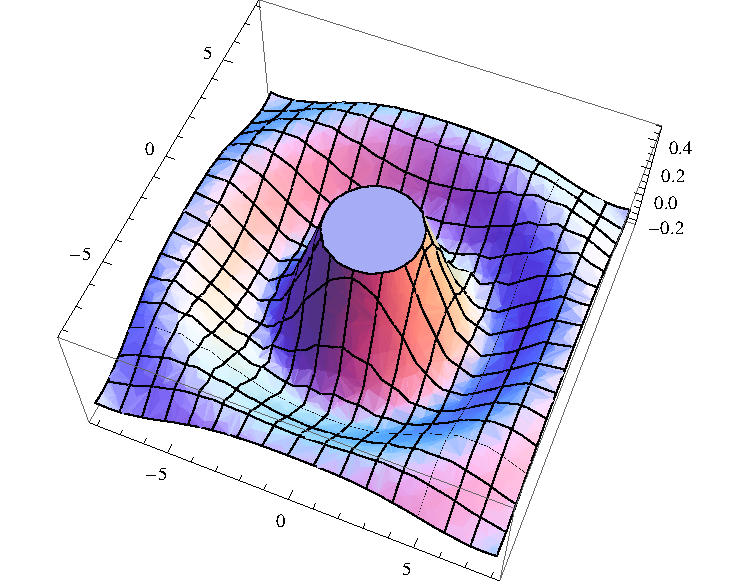
\includegraphics[width=7cm]{EjemploFigura.pdf}
	\label{EtiquetaFigura}
	\medskip
	\caption*{\emph{Nota}: Esta es una nota explicativa\\ sobre la imagen (opcional)}
\end{figure}

\noindent En la Tabla \ref{EtiquetaDeLaTabla} ...
\begin{table}[h!]
\caption{Título de la tabla}
\centering
\begin{tabular}{c|c|c}
	& 1 & 2 \\
	\hline
	A &  &  \\
	\hline
	B &  &  \\
\end{tabular}
\label{EtiquetaDeLaTabla}
\medskip
\caption*{\emph{Nota}: Nota de la tabla (opcional)}
\end{table}


\section{Cómo citar}\label{EtiquetaDeSeccion23}
\begin{itemize}
	\item \textbf{Citas cortas} (hasta 40 palabras):Se incluyen en el texto con comillas.
	\item \textbf{Citas largas} (más de 40 palabras): Se escriben en párrafo separado sin comillas.
\end{itemize}

\subsection{\emph{apacite}}
\noindent Para citar en formato APA, puede usarse el paquete \emph{apacite}. Algunas opciones de citación pueden hacerse con los comandos que se presentan en la Tabla \ref{ComandosApacite}; puede consultar \cite{meijer2013apacite} para la información completa de la documentación del paquete.

\begin{table}[h!]
\caption{Algunos comandos del paquete \emph{apacite} }
\centering
\scriptsize
	\begin{tabular}{ll}
		\hline
		\textbf{Texto plano}&\textbf{Produce}\\
		\hline
		\verb|\cite{RudinKEY} afirma que|&\cite{RudinKEY} afirma que \\
		\verb|\cite[p.123]{RudinKEY} afirma que|&\cite[p.123]{RudinKEY} afirma que\\
		\verb|Como se pude ver en  \citep{RudinKEY}|&Como se pude ver en  \citep{RudinKEY}\\
		\verb|\citealp{RudinKEY}|&\citealp{RudinKEY}\\
		\verb|Ver Rudin \citeyearpar {RudinKEY}|&Ver Rudin \citeyearpar {RudinKEY}\\
		\verb|Como se pude ver en  \citet{RudinKEY}|&Como se pude ver en  \citet{RudinKEY}\\
		\verb|Como se pude ver en  \citetext{RudinKEY}|&Como se pude ver en  \citetext{RudinKEY}\\
		\verb|Puede consultar \citeauthor {RudinKEY}|&Puede consultar \citeauthor {RudinKEY}\\
		\verb|Confrontar Lamport \citeyear {RudinKEY}|&Confrontar Lamport \citeyear {RudinKEY}\\
		\hline
	\end{tabular}
\label{ComandosApacite}
\medskip
\caption*{\emph{Nota}: Tabla extraída de \citet[p. 50]{WunschKEY}.}
\end{table}

\subsection{Citas textuales}

\begin{itemize}
  \item \textbf{Narrativa}.

  \underline{Cita corta}.

   Como menciona \cite{apostol1976analisis}, ``\emph{la idea de expresar geométricamente los números complejos como puntos de un plano fue formulada por Gauss en su disertación de 1799 e, independiente, por Argand en 1806.}'' (p. 21). Sin embargo ...

  \underline{Cita larga}

  Como menciona \cite{apostol1976analisis}:
  \begin{itemize}
    \item [] La idea de expresar geométricamente los números complejos como puntos de un plano fue formulada por Gauss en su disertación de 1799 e, independiente, por Argand en 1806. Más tarde Gauss ideó la expresión un tanto desafortunada de ''número complejo''. Los números complejos admiten otras representaciones geométricas. En vez de utilizar puntos de un plano, se pueden utilizar puntos de otras superficies. (p. 22)
  \end{itemize}



  \item \textbf{Con paréntesis}.

  Los números complejos, pueden representarse como puntos de un plano, ``\emph{la idea de expresar geométricamente los números complejos como puntos de un plano fue formulada por Gauss en su disertación de 1799 e, independiente, por Argand en 1806.}'' \cite[p. 21]{apostol1976analisis},

\end{itemize}

\subsection{Citas parafraseadas}
\begin{itemize}
  \item \textbf{Narrativa}.

  De acuerdo a \cite{apostol1976analisis}, otra representación geométrica de los números complejos es la llamada \textbf{proyección estereográfica} que consiste en proyectar los puntos del polo norte de la esfera sobre el plano tangente en el polo de dicha esfera. (p. 22)
  \item \textbf{Con paréntesis}.

  Otra representación geométrica de los números complejos es la llamada \textbf{proyección estereográfica} que consiste en proyectar los puntos del polo norte de la esfera sobre el plano tangente en el polo de dicha esfera.\cite[p. 22]{apostol1976analisis}
\end{itemize}




\chapter{Nombre del Capítulo 3 (Metodología)}
\markboth{CAPÍTULO 3: NOMBRE DEL CAPÍTULO 3}{\small CAPÍTULO 3: NOMBRE DEL CAPÍTULO 3}
\label{Metodologia}

\noindent En este capítulo...

%------------------------------------------------------------------------------------------------------------
\section{Nombre de la Sección} \label{EtiquetaDeSeccion31}
\noindent Texto...

\begin{table}[h!]
\caption{Algunas funciones complejas }
\centering
\begin{tabular}{ll|r}
	&\textbf{$w=f(z)$}&\textbf{Región en que $w$ está definida}\\
	\cline{2-3}
	a)&$\displaystyle w=2z$&Todo el plano\\
	\cline{2-3}
	b)&$\displaystyle w=e^{|z|}$&Todo el plano\\
	\cline{2-3}
	c)&$\displaystyle w=2i|z|^2$&Todo el plano\\
	\cline{2-3}
	d)&$\displaystyle w=\frac{z+3i}{z^2+9}$ &Todo el plano excepto $\pm 3i$
\end{tabular}
\label{EtiquetaDeLaTabla2}
\medskip
\caption*{\small  \emph{Nota}: Tabla extraída de \citet[p. 50]{WunschKEY}.}
\end{table}


%


\chapter{Nombre del capítulo 4 (Desarrollo)}
\markboth{CAPÍTULO 4. NOMBRE DEL CAPÍTULO 4}{\small CAPÍTULO 4. NOMBRE DEL CAPÍTULO 4}
\label{Desarrollo}

\noindent En este capítulo se expone ...

%------------------------------------------------------------------------------------------------------------
\section{Nombre de la Sección A} \label{EtiquetaDeSeccion41}
\noindent Texto...

%------------------------------------------------------------------------------------------------------------
\section{Nombre de la sección B} \label{EtiquetaDeSeccion42}
\noindent Texto...


%\chapter*{Resultados}
\markboth{ANÁLISIS E INTERPRETACIÓN DE RESULTADOS}{\small ANÁLISIS E INTERPRETACIÓN DE RESULTADOS}
\label{Resultados}
\addcontentsline{toc}{chapter}{Análisis e interpretación de resultados}

\noindent \textcolor[rgb]{0,0,1}{
	En este capítulo debes construir interpretaciones a partir de los datos obtenidos en la etapa anterior; para esto tendrás que explicar la validez del modelo metodológico aplicado y demostrar la objetividad de los instrumentos de medición utilizados.}

\noindent \textcolor[rgb]{0,0,1}{
	Te recomendamos que primero reportes de manera sintética los resultados y principales hallazgos de tu investigación, y después los describas de manera minuciosa, pero resérvate las conclusiones y recomendaciones para sus respectivos apartados. Relacionar siguiendo los objetivos específicos Se presentan los resultados logrados en forma cuantitativa. Para los objetivos que estén en vías de logro, o que no se lograron, se presentarán las causas correspondientes que expliquen la situación de cada uno según sea el caso.}

\noindent \textcolor[rgb]{0,0,1}{
	Esta sección se termina con una presentación de “Antes y Después”, mostrando los aspectos cuantitativos de cada problema resuelto. Esta parte puede incluir: tablas, gráficas, fotos, videos, etc.}\newpage

\noindent \textcolor[rgb]{0,0,1}{
	En la segunda, se reporta para que demuestres, que el proyecto fue rentable o benéfico para la empresa. Para tal efecto, se podrán utilizar demostraciones de: costo-­‐beneficio, diagramas de flujo de efectivo, rentabilidad por medio de la tasa de retorno de inversión. En esta parte deberán tomarse en cuenta todas las inversiones efectuadas, tales como: las adquisiciones, percepciones incluyendo las del pasante, horas estándar invertidas, pruebas, etc.}

%\chapter*{Conclusiones}
\markboth{CONCLUSIONES Y TRABAJOS FUTUROS}{\small CONCLUSIONES Y TRABAJOS FUTUROS}
\addcontentsline{toc}{chapter}{Conclusiones y trabajos futuros}

\noindent \textcolor[rgb]{0,0,1}{
	Este apartado trata de manera puntual la condición de aceptación o rechazo de la hipótesis. También se deberá referir los hechos más relevantes durante la investigación y los hallazgos o aportes principales, apoyados por la argumentación sobre el valor del estudio.}

\noindent \textcolor[rgb]{0,0,1}{
	A continuación presentamos ejemplos de cómo iniciar la redacción de las conclusiones:
	\begin{itemize}
		\item Con base en los resultados obtenidos en la presente investigación, se llegó a las siguientes conclusiones [\ldots]
		\item En cuanto a la teoría que respalda los resultados es importante enfatizar que [\ldots]
		\item La hipótesis quedó plenamente demostrada, pues los hallazgos permitieron confirmar [\ldots]
		\item El marco metodológico adoptado indica que [\ldots].
	\end{itemize}
}



\noindent \textbf{Trabajos Futuros}

\noindent \textcolor[rgb]{0,0,1}{
	Proponer trabajos futuros que se pueden realizar. Numerado, viñetas o texto.}

\noindent \textcolor[rgb]{0,0,1}{
	Ejemplo:\newline
	Como trabajos futuros que se pueden proponer y realizar, son los siguientes: 
	\begin{enumerate}
		\item Plantear el problema de distribución como uno en el área de Teoría de Redes.
		\item Considerar escalón más al modelo, que representaría la distribución desde las zonas de extracción a las refinerías.
		\item Subir a alguna plataforma especializada la base de datos creada en esta investigación.
		\item Proponer un modelo multi objetivo en la distribución de derivados del petróleo.
	\end{enumerate}
}



% ------------------------------------------------------------------------
%\chapter*{Recomendaciones (Opcional)}
\markboth{RECOMENDACIONES}{\small RECOMENDACIONES}
\addcontentsline{toc}{chapter}{Recomendaciones (Opcional)}

\begin{enumerate}
  \item
  \item
\end{enumerate}




%\chapter*{Abreviaturas}
\markboth{ABREVIATURAS}{\small ABREVIATURAS}
\addcontentsline{toc}{chapter}{Abreviaturas}

\begin{tabular}{ll}
  UAT & Universidad Aut\'onoma de Tlaxcala
\end{tabular}



\appendix
%\chapter*{Apéndice (Opcional)}
\markboth{APÉNDICE}{\small APÉNDICE}
\addcontentsline{toc}{chapter}{Apéndice (Opcional)}
\label{Apendice}

\noindent \textbf{$($M. Asadi, etc. \cite{ASSOVARH2009}$)$}
Sea $E$ un espacio  de Banach real. Un subconjunto $\mathcal{P}\subset E$, no vacío, cerrado y convexo es llamado un \emph{cono} en $E$ si satisface lo siguiente:
\begin{itemize}
	\item [$i)$] $\mathcal{P}$ es cerrado, no vacío y $\mathcal{P}\neq \{0\}$,
	\item [$ii)$] $a,b\in \mathbb{R}$, $a,b\geq 0$ y $x,y\in \mathcal{P}$ implica que $a x+ b y \in \mathcal{P}$,
	\item [$iii)$] $x\in \mathcal{P}$ y $-x\in \mathcal{P}$ implica que $x=0$.
\end{itemize}


% ------------------------------------------------------------------------
\bibliographystyle{apacite}
\bibliography{ref}
\end{document}
% ------------------------------------------------------------------------
